\section{Control Supervisado}
{\begin{small}%
\begin{flushright}%
\it
Entiende el problema y tendrás la solución
\end{flushright}%
\end{small}%
\vspace{.5cm}}
El presente proyecto de tesis consistió en un estudio y extensión del método previamente propuesto por Daniel Ciolek en su tesis de doctorado[REF PAPER?]. Más precisamente, se trató de analizar carencias del algoritmo de exploración on-the-fly para problemas de Supervisory Control, cuya propiedad central era de tipo Non-blocking, y posteriormente analizados los problemas afrontarlos con una nueva especificación e implementación del algoritmo.
\\
Un problema de Control Supervisado consiste en un Sistema de Eventos Discreto (DES) con un subconjunto de sus estados marcados. Un factor clave de estos problemas es que el DES se presenta de forma compacta, de forma modular tal que la composición paralela de múltiples componentes den lugar a la DES de interés.
\\

\subsection{Caso de estudio}
A continuación se presenta un ejemplo sobre el cual aplicaremos nuestro algoritmo a lo largo de la presentación. 

Imaginemos un negocio del cual modelamos 3 componentes: La cuenta de dinero, la estación de ventas de productos terminados, y la estación de compra de materia prima y ensamblaje de productos.

La cuenta de dinero puede estar vacía o con dinero, no contamos cuanto dinero hay, pero sabemos que en caso de estar vacía no se pueden comprar nuevas materias primas. También podemos elegir al momento de comprar nuevos materiales si queremos gastar todo el dinero que hay en la cuenta o solo gasta una parte.

La estación de ensamble puede necesitar comprar nuevos materiales, y una vez que los recibe necesita un tiempo no controlable hasta finalizar el próximo producto, momento en el que el mismo se transfiere a la estación de ventas.

La estación de ventas, cuando tiene un producto para vender, tarda un tiempo no controlable hasta que llega un cliente que compra el producto, momento en el que la cuenta del negocio guarda la plata y seguramente no está vacía.

Mostramos en la figura~\ref{fig:modelos} un LTS (Labeled transition system) para cada uno de los componentes descriptos.


\begin{figure}[htb]
	\begin{center}
	\makebox[\linewidth][c]{%
	\begin{subfigure}[t]{.7\textwidth}
		\centering
		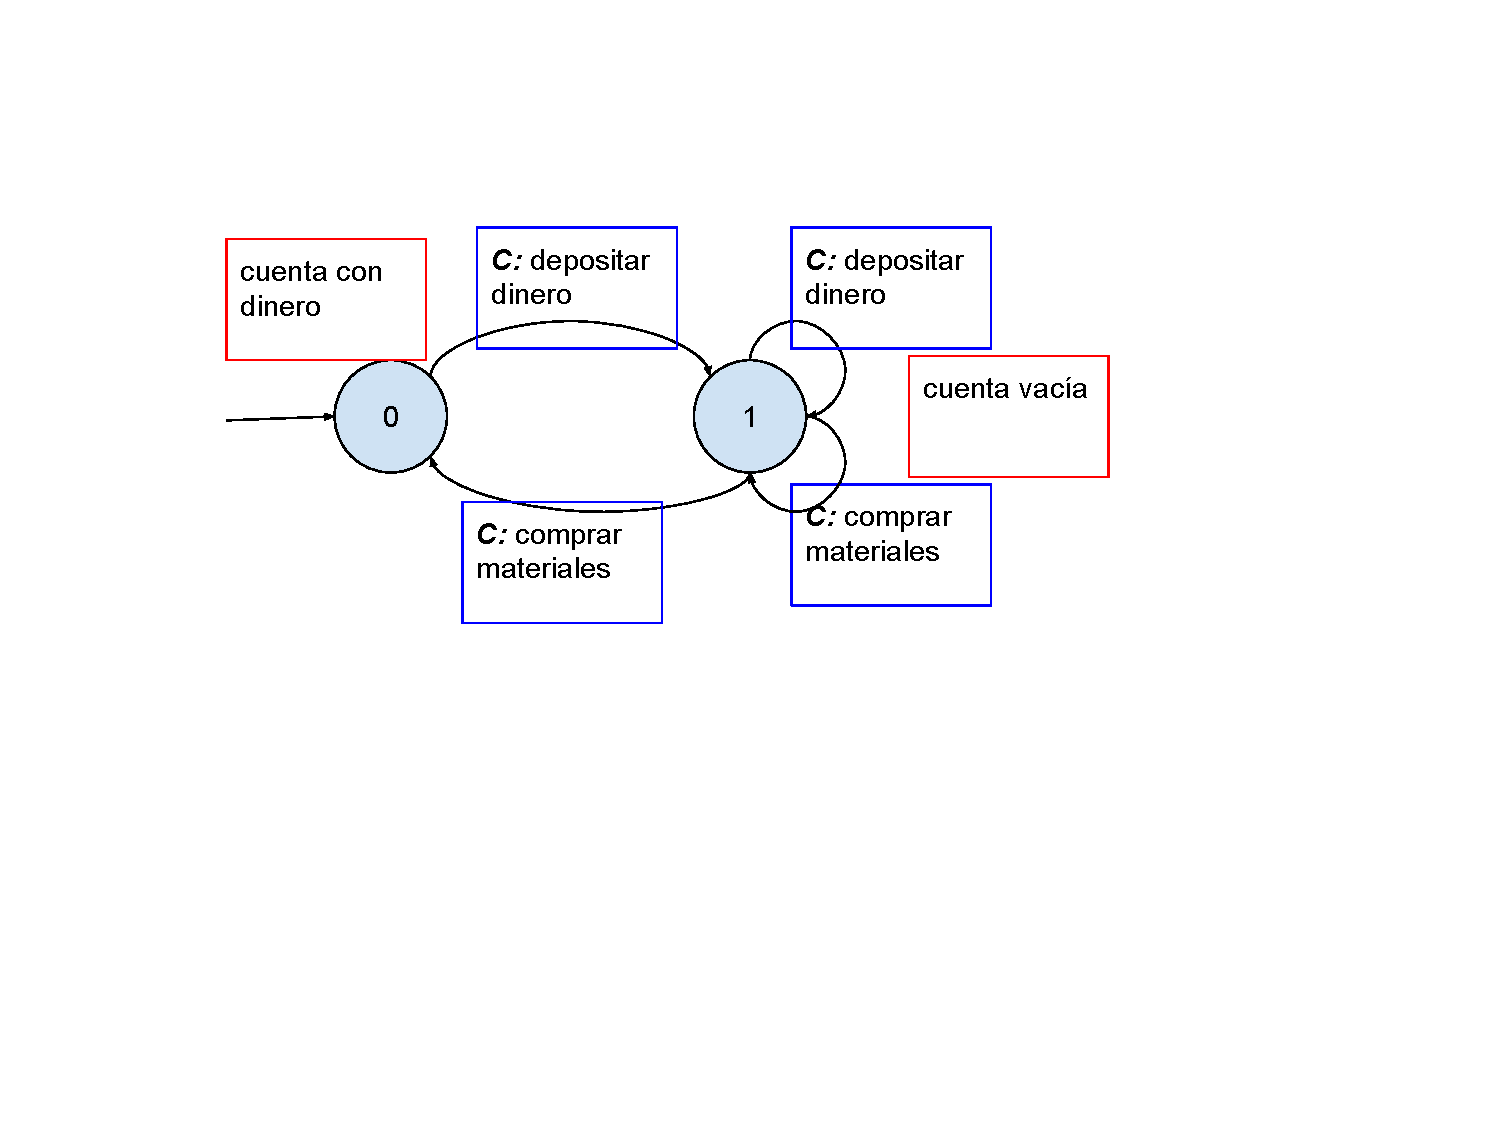
\includegraphics[width=\linewidth]{figures/ModeloCuentaBanco.pdf}  
		\caption{Cuenta bancaria}
		\label{fig:ModeloBanco}
	\end{subfigure}
	\begin{subfigure}[t]{.7\textwidth}
		\centering
		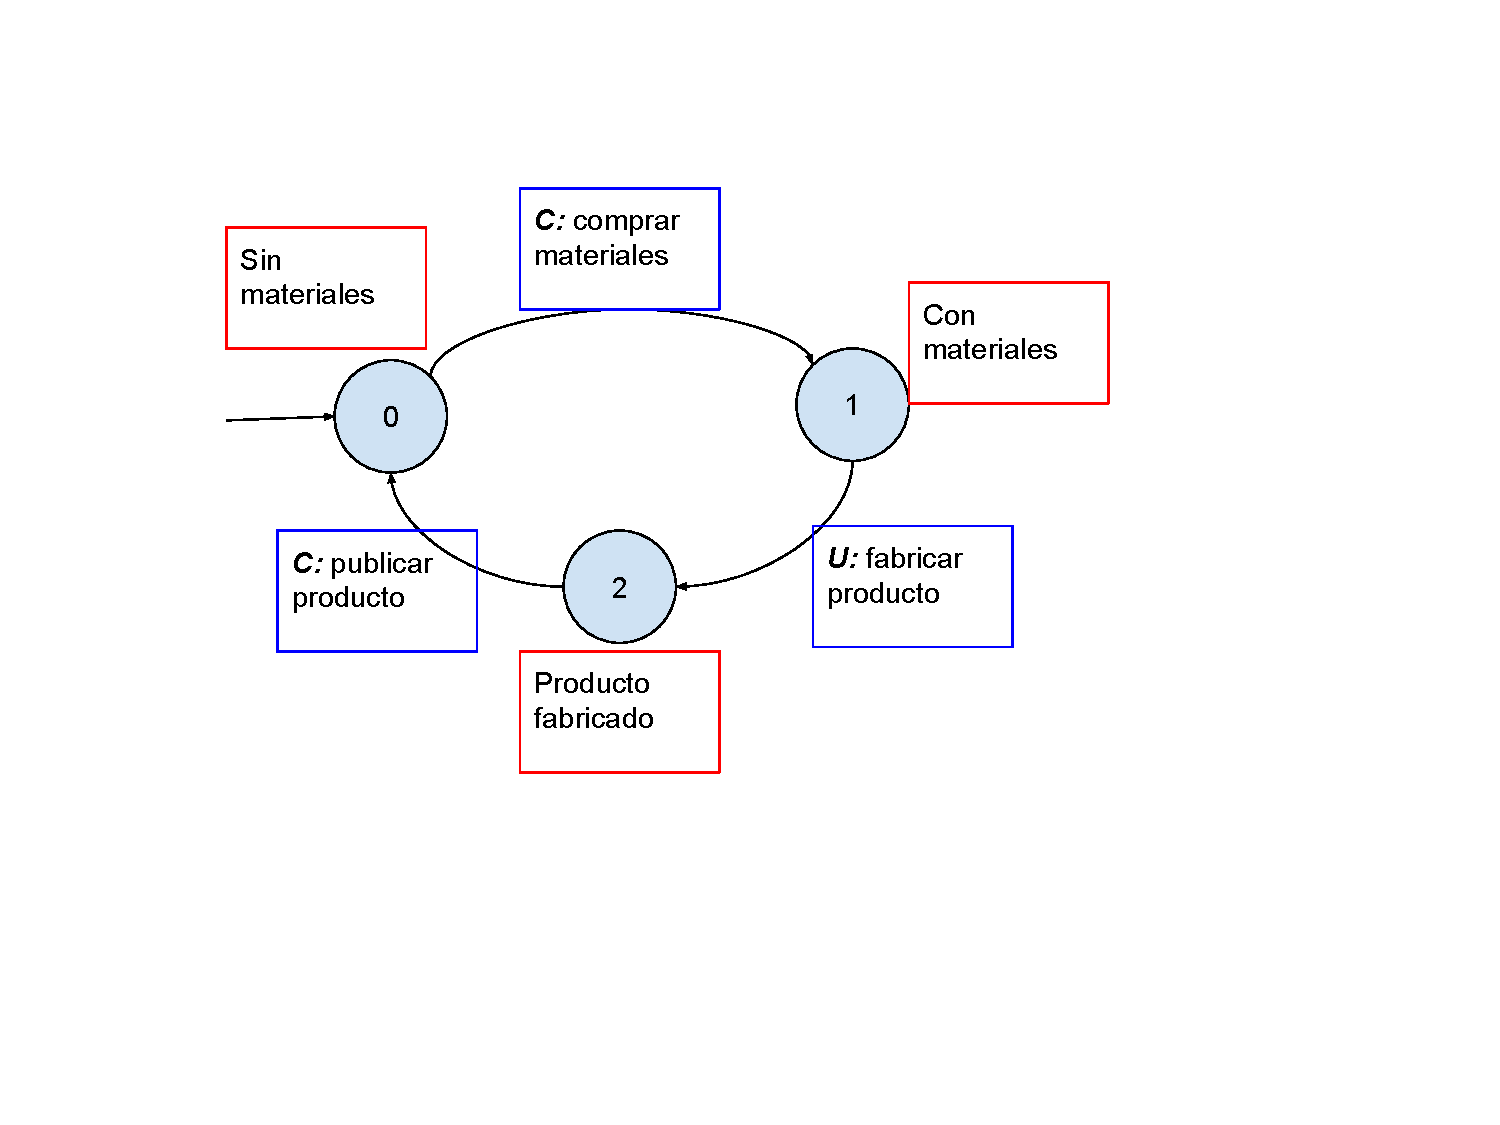
\includegraphics[width=\linewidth]{figures/ModeloEnsamblaje.pdf}  
		\caption{Estacion de ensamblaje}
		\label{fig:modeloEnsamblajes}
	\end{subfigure}
	}
	\makebox[\linewidth][c]{%
	\begin{subfigure}[t]{.7\textwidth}
		\centering
		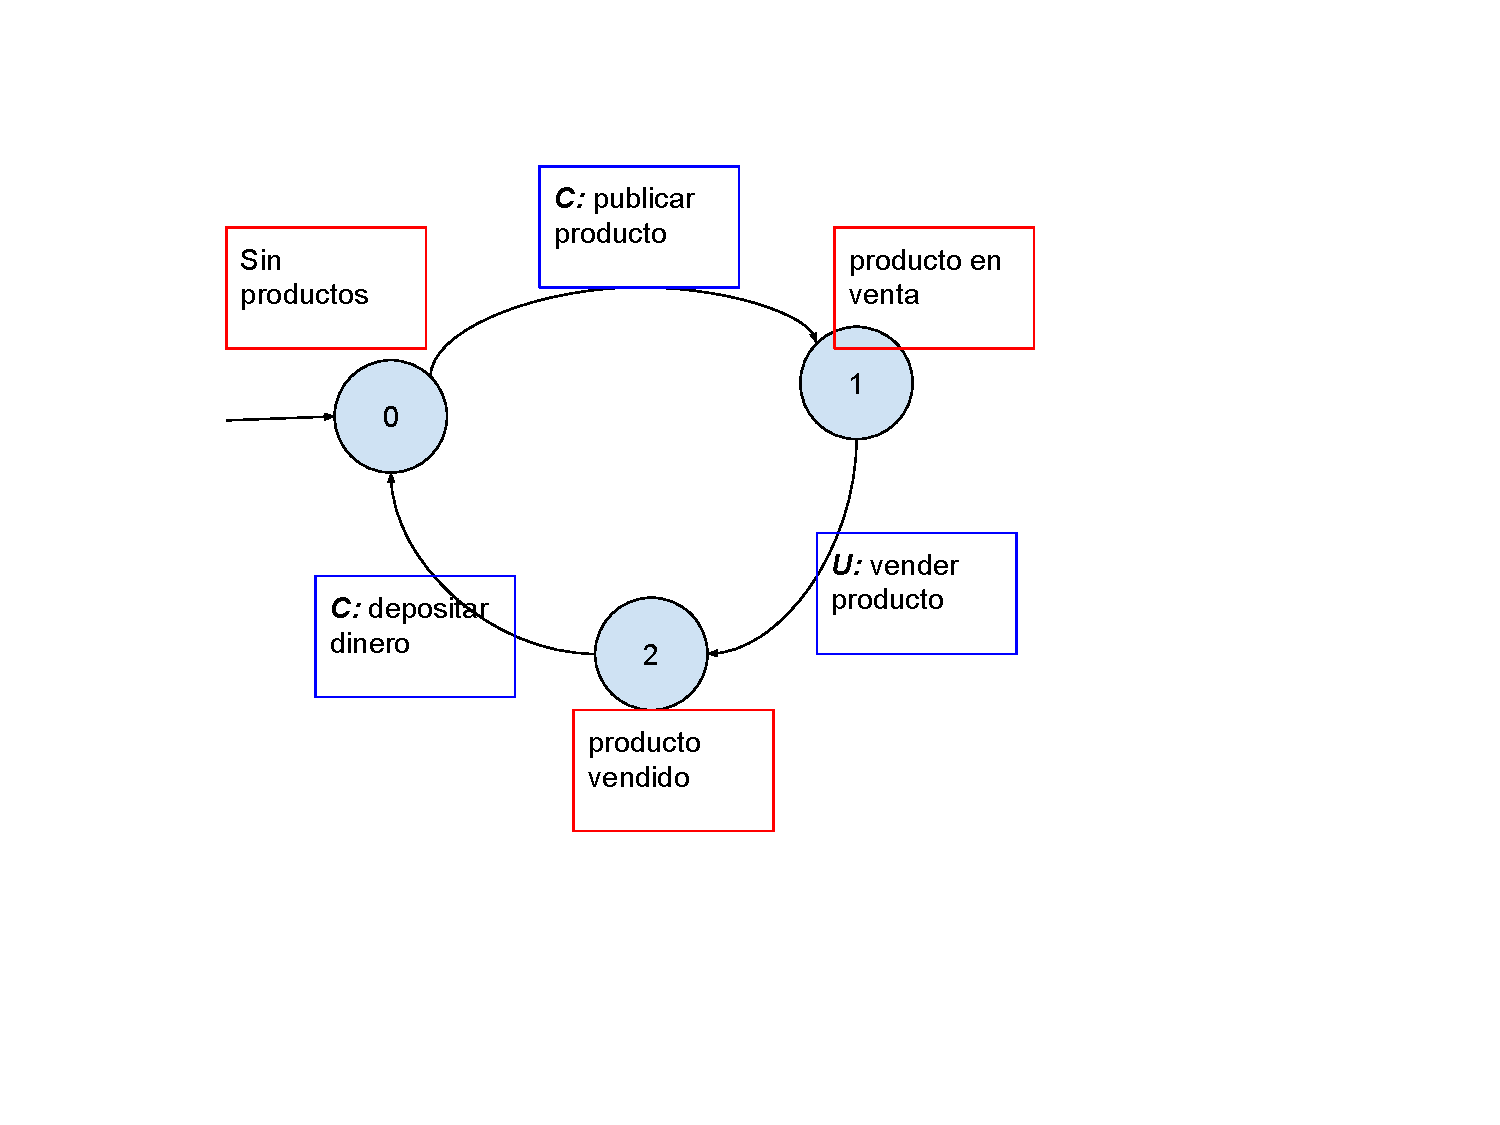
\includegraphics[width=\linewidth]{figures/ModeloVentas.pdf}  
		\caption{Estacion de ventas}
		\label{fig:modeloVentas}
	\end{subfigure}
	\begin{subfigure}[t]{.7\textwidth}
	\centering
	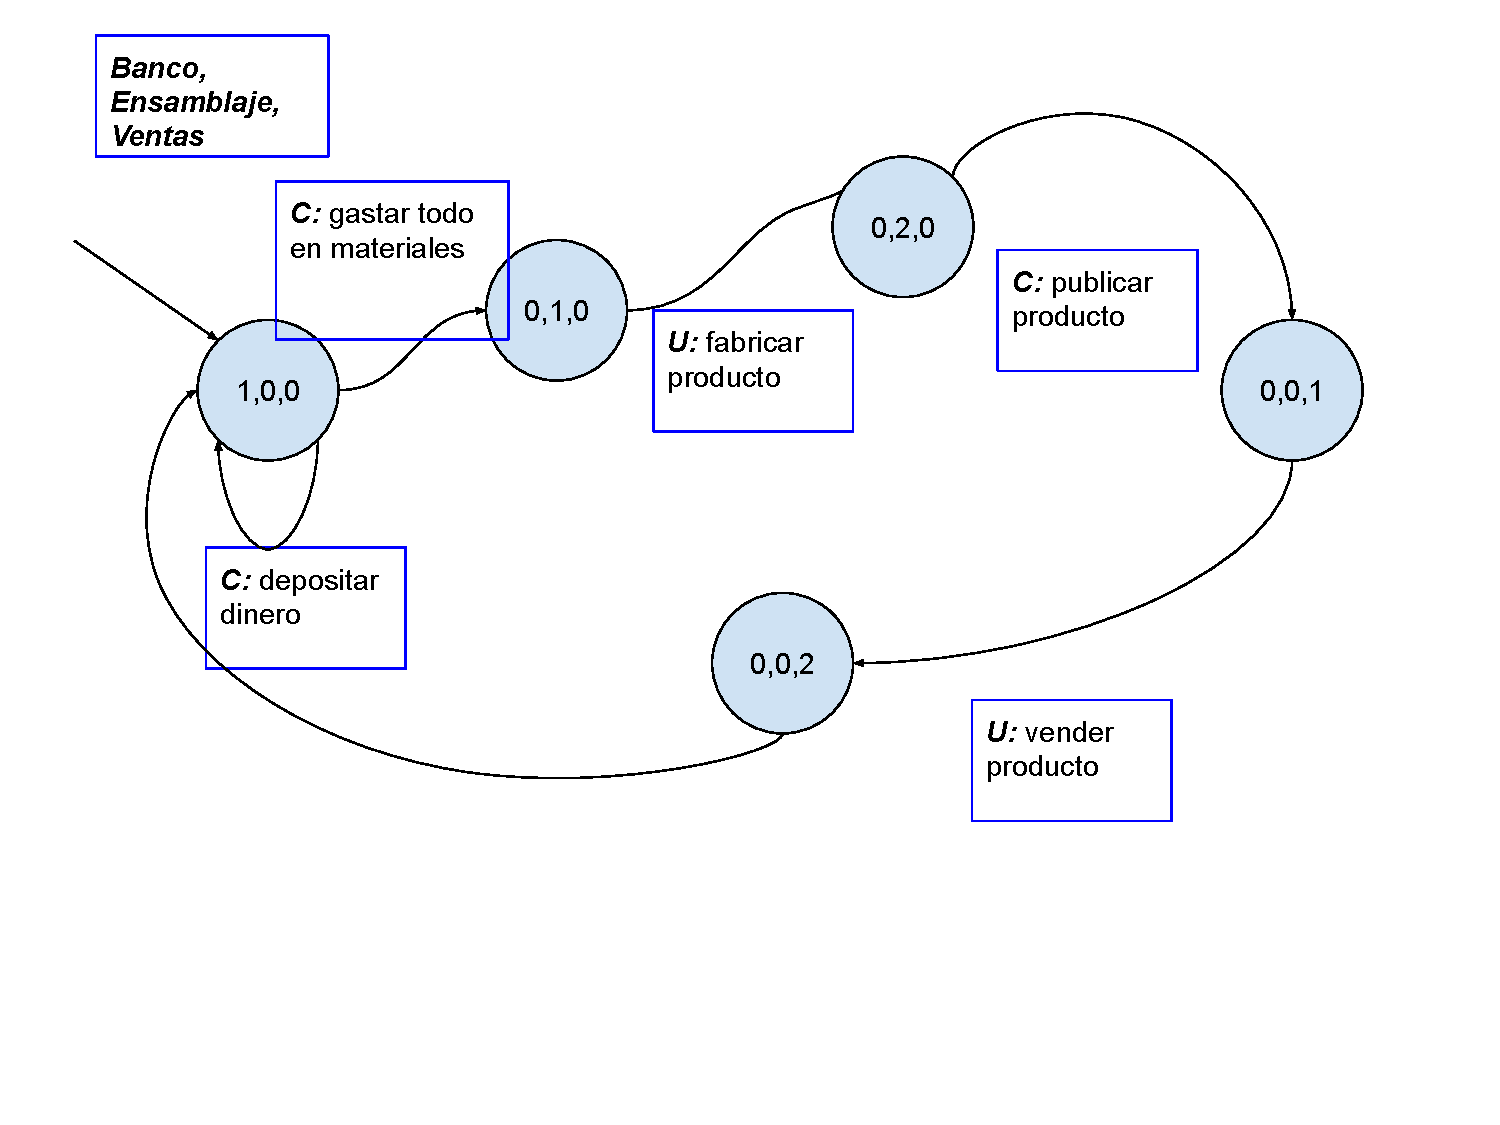
\includegraphics[width=\linewidth]{figures/ModeloCompuestoSin2Caminos.pdf}  
	\caption{Composición de los componentes}
	\label{fig:compuesto}
	\end{subfigure}
	}
	\caption{Modelo de ejemplo}
	\label{fig:modelos}
	\end{center}
\end{figure}



\subsection{Controlador objetivo}
DESCRIPCION nonblocking
\\

\subsection{Exploración on-the-fly}
Problema explosión exponencial: Componer todo vs BFS
\\